\section{SIMP Implementation in Julia}

The SIMP algorithm consists of two main loops. The inner loop consists of the optimization process facilitated by the Method of Moving Asymptotes

\subsection{``King Me'': Avoiding the Checkerboard Problem}\label{sec:checkerboarding}

If one were to optimize conductive material placement to increase heat transfer on a standard rectangular grid, a simplistic solution would be to create a grid of alternating material types in each adjacent rectangle, like a checkerboard. This way, the heat is always flowing to adjacent cells. While this may indeed increase heat transfer, it doesn't necessarily decrease the average temperature in our object (or transfer the heat towards the heat-sink). Hence, avoiding this non-physical checkerboard solution is of concern.

\begin{figure}
	\centering
	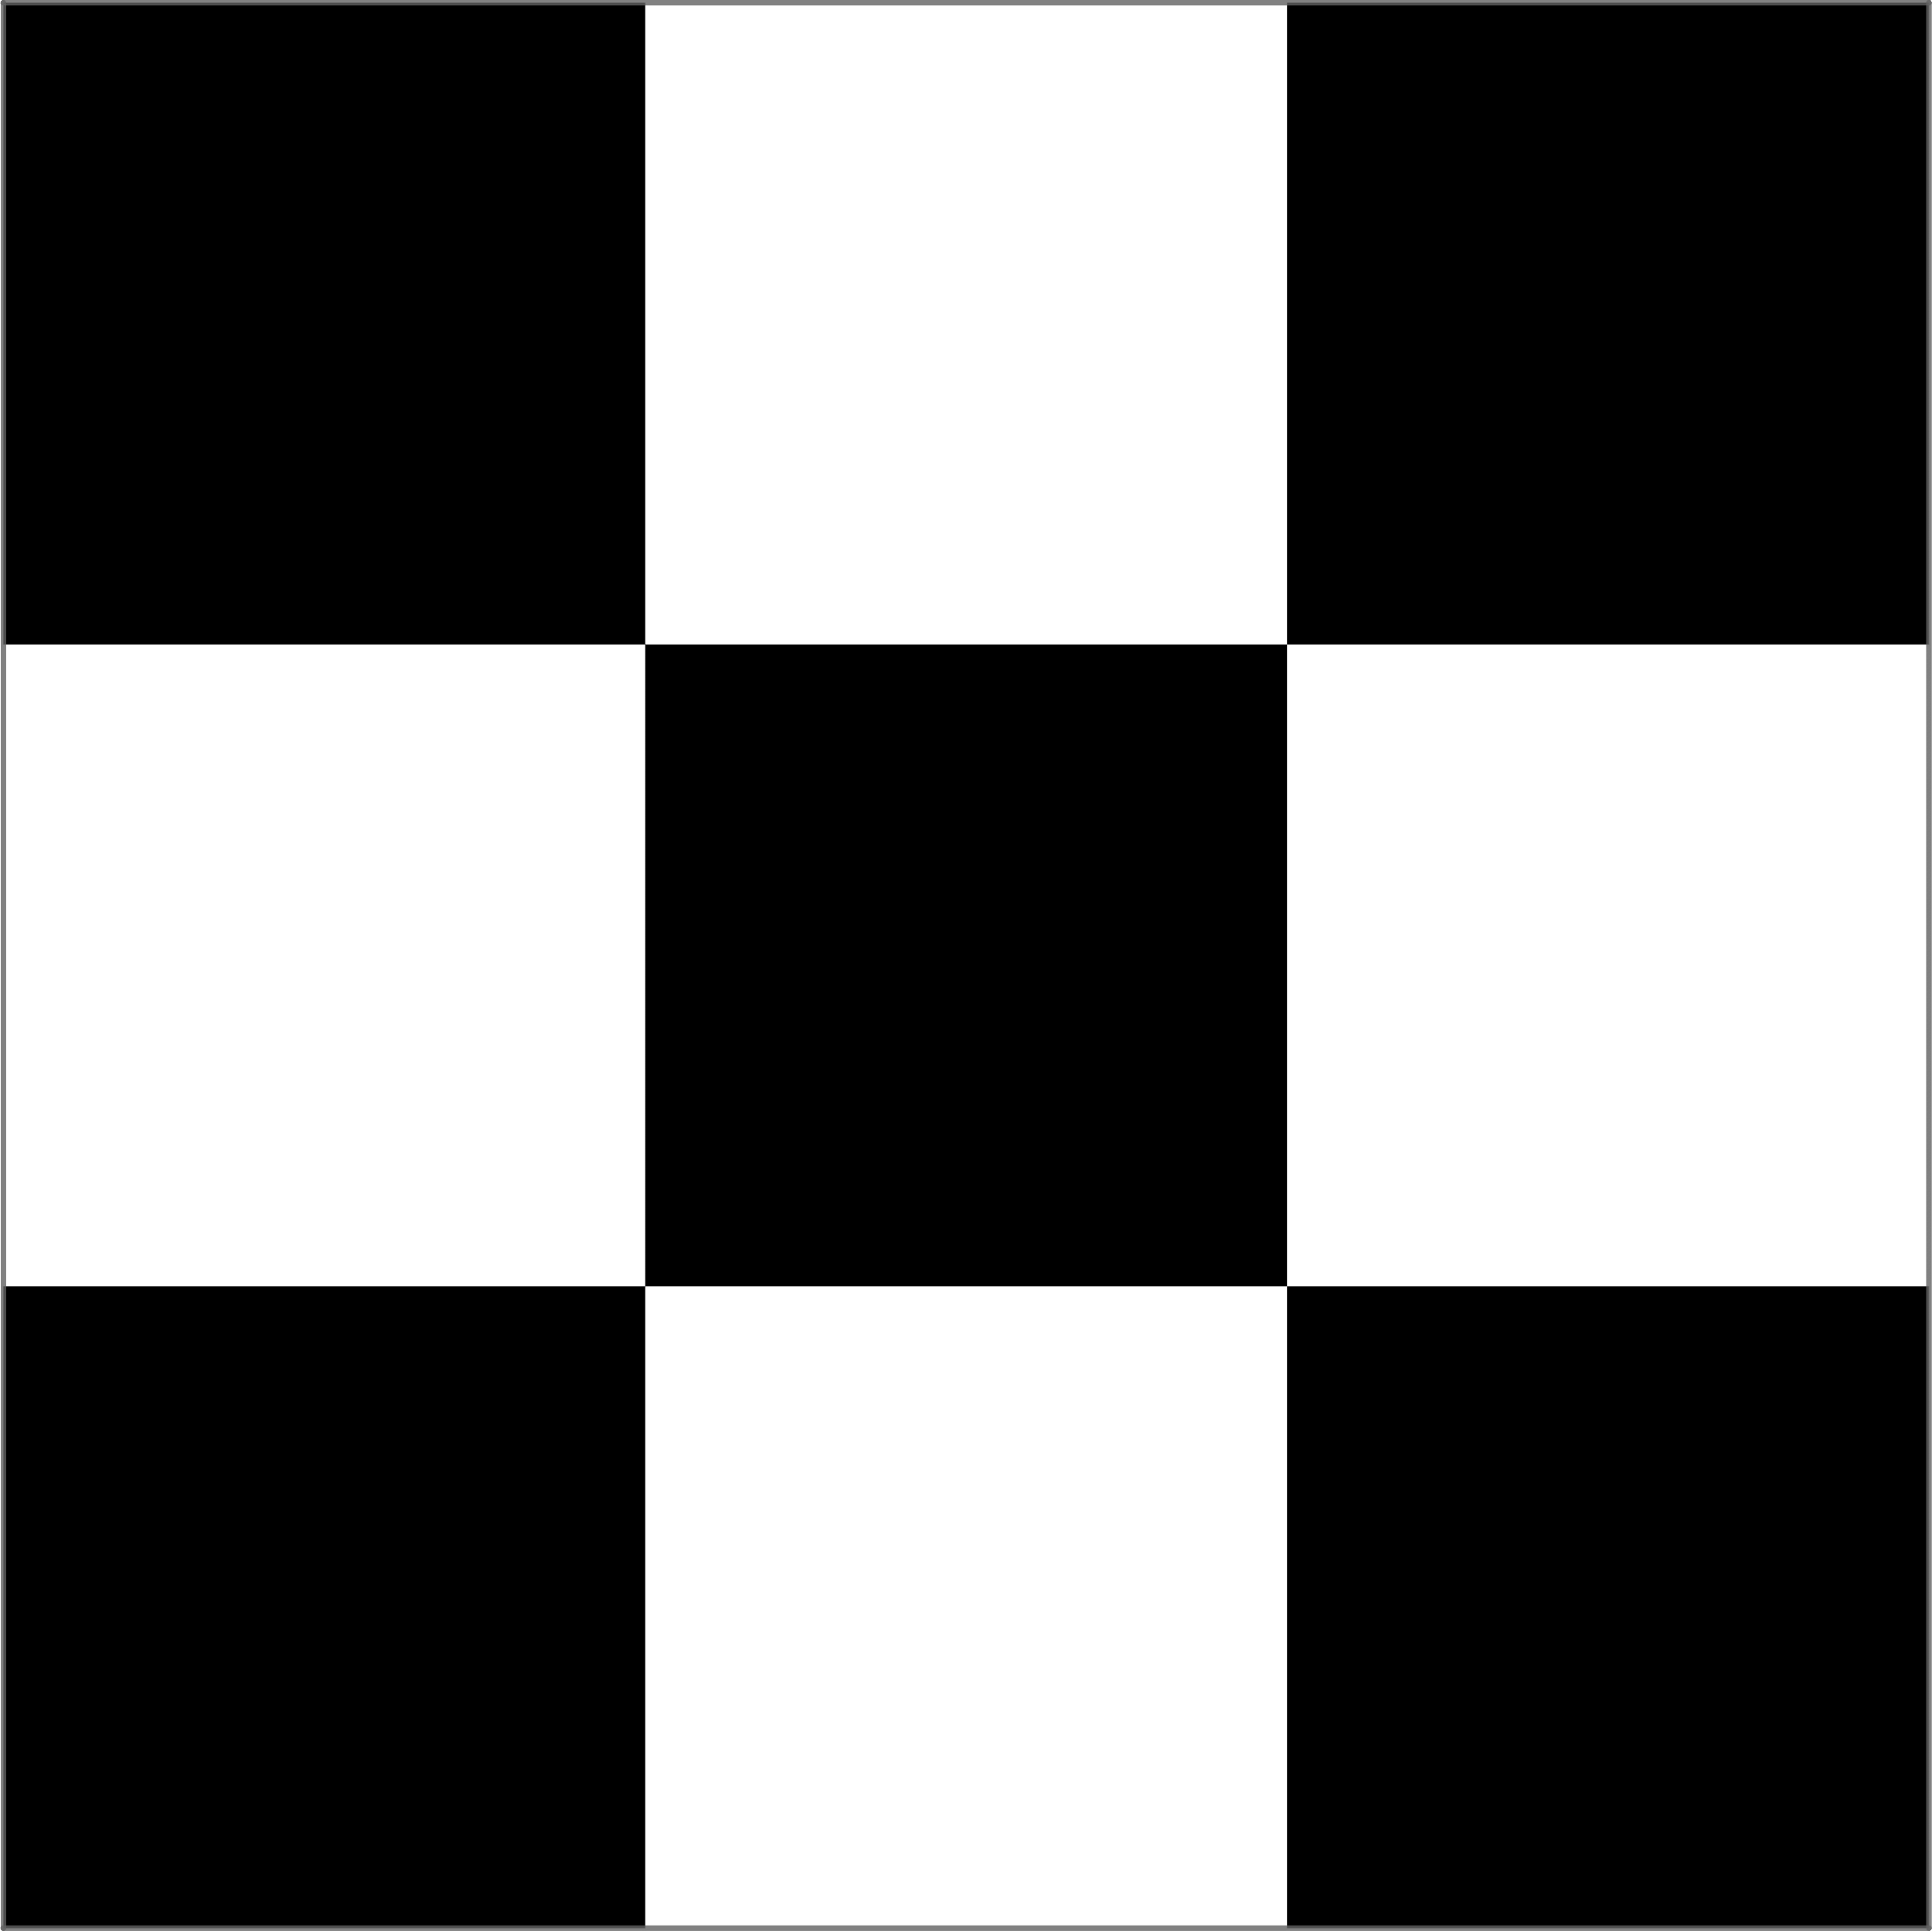
\includegraphics[width=0.4\textwidth]{Chapter_II_SIMP_Optimization/Images/3x3-Checkerboard.png}
	\caption[Checkerboard Pattern]{A checkerboard pattern result on a 3-by-3 control volume grid. The black spaces represent areas where $\eta=1$ and the white spaces represent areas where $\eta=0$ in \eqref{eqn:penalization}. This results in adjacent regions of alternating thermal conductivites $k_+$ and $k_0$, artificially maximizing heat transfer between control volumes.}
	\label{fig:3x3-Checkerboard}
\end{figure}

\begin{figure}
	\centering
	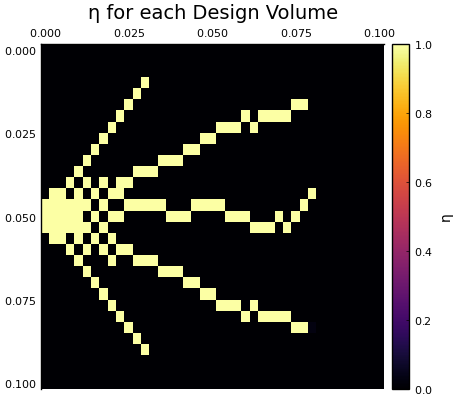
\includegraphics[width=0.8\textwidth]{Chapter_II_SIMP_Optimization/Images/SIMP-Example-Checkerboarding.png}
	\caption[Checkerboard Result in Practice]{Output of SIMP algorithm for $30\times 40$ temperature control volumes. Notice the local checkerboarding around $(0.05,0.015)$.}
	\label{fig:SIMP-Checkerboard}
\end{figure}

In order to solve the heat equation \eqref{eqn:HeatEq}, we employ the Finite Volume Method (described earlier). This involves splitting up our space into a finite number of control volumes. The checkerboard pattern emerges when the solution of our optimization process converges to a 1---0 structure which has some meshes that successively belong to the $\Omega_0$ and $\Omega_+$ sets (i.e.: adjacent grid volumes have alternating thermal conductivites). As a result, the heat transfer within the structure between $k_+$ and $k_0$ regions is maximized, artificially increasing the impact of adding $k_+$ material on the temperature $T$, which in turn minimizes the objective function in \eqref{SIMP-Optimization-Problem} \cite{Versteeg2007}. Typically, this pattern occurs locally but then spreads throughout the entire structure through successive iterations of the optimization process. However, in the real world, these checkerboard placements of our conductive materials do not actually have the effect of lowering the average temperature in structures. In fact, the checkerboard example in Figure \ref{fig:3x3-Checkerboard} doesn't even direct heat towards the heat-sink on the left wall of the structure.

In order to avoid obtaining checkerboard solutions from our optimization process, we employ two separate staggered grids for our temperature and design variables (see Figure \ref{fig:grids}). We need to employ some extra equations in order to translate between design and temperature variables, but this strategy helps solve the issue of convergence to checkerboard solutions.